\documentclass[aps,superscriptaddress,nofootinbib,floatfix,notitlepage]{revtex4-1}
\pdfoutput=1
\usepackage{amsmath}
\usepackage{amssymb}
\usepackage{bm}
\usepackage{graphicx}
\usepackage{hyperref}
\usepackage[utf8x]{inputenc}
\usepackage{lmodern}
\usepackage{xspace}
%\usepackage[punctsep]{collref}

\newcommand{\HEPfit}{\texttt{HEPfit}\xspace}

\begin{document}

\title{\HEPfit: a Code for the Combination of Indirect and Direct
  Constraints\\ on High Energy Physics Models. \\
  v1.0: Precision Electroweak Observables, Higgs Signal Strengths,\\ and Flavour Violation in the
  Standard Model and Beyond
  \vspace*{0.5cm}
%  \begin{figure}[htb!]
%   \begin{center}
% %  \includegraphics[width=0.13\textwidth]{logo}
%   \end{center}
% \end{figure}
% \vspace*{-0.8cm}
}

\collaboration{
%\begin{figure}[h!]
  %\begin{center}
  %\includegraphics[width=0.13\textwidth]{logo}
  %\end{center}
 %\end{figure}
\HEPfit Collaboration
}
%\homepage{http://www.susyfit.org} 
\homepage{http://hepfit.roma1.infn.it} 
%\affiliation{}
\author{M.~Ciuchini}
\affiliation{INFN,  Sezione di Roma Tre, Via della Vasca Navale 84, I-00146 Roma, Italy}
\author{J.~de Blas}
\affiliation{INFN, Sezione di Roma, Piazzale A. Moro 2, I-00185 Roma, Italy}
\author{D.~Chowdhury}
\affiliation{INFN, Sezione di Roma, Piazzale A. Moro 2, I-00185 Roma, Italy}
\author{O.~Eberhardt}
\affiliation{INFN, Sezione di Roma, Piazzale A. Moro 2, I-00185 Roma, Italy}
\author{M.~Fedele}
\affiliation{INFN, Sezione di Roma, Piazzale A. Moro 2, I-00185 Roma, Italy}
\author{E.~Franco}
\affiliation{INFN, Sezione di Roma, Piazzale A. Moro 2, I-00185 Roma, Italy}
\author{S.~Mishima}
\affiliation{Institute of Particle and Nuclear Studies, KEK, Tsukuba 305-0801, Japan}
\author{A.~Paul}
\affiliation{INFN, Sezione di Roma, Piazzale A. Moro 2, I-00185 Roma, Italy}
\author{L.~Reina}
\affiliation{Physics Department, Florida State University, Tallahassee, FL 32306-4350, USA}
\author{L.~Silvestrini}
\affiliation{INFN, Sezione di Roma, Piazzale A. Moro 2, I-00185 Roma, Italy}
\author{M.~Valli}
\affiliation{SISSA, via Bonomea 265, I-34136 Trieste, Italy and INFN, Sezione di Trieste, via Valerio 2, I-34127 Trieste, Italy}
\begin{abstract}
\HEPfit is a flexible %open-source
tool which, given the Standard Model or any extension, allows to \textit{i)} fit the model
parameters to a given set of experimental observables;
\textit{ii)} obtain predictions for observables.
\HEPfit can be used either in Monte Carlo mode, to perform a Bayesian Markov Chain Monte Carlo
analysis of the given model, or as a library, to obtain predictions of
observables for a given point in the parameter space of the model, allowing our computational tool to be used in
any statistical framework. In the present version, Electroweak Precision Observables have been implemented
in the Standard Model and in several New Physics scenarios.


\end{abstract}
 
\maketitle



%%%%%%%%%%%%%%%%%%%%%%%%%%%%%%%%%%%%%
\section{Introduction}
%%%%%%%%%%%%%%%%%%%%%%%%%%%%%%%%%%%%%

Searching for New Physics (NP) in the LHC era requires combining
experimental and theoretical information from many sources to optimize
the NP sensitivity. NP searches, even in the absence of a positive
signal, provide useful information which puts constraints on the
viable parameter space of any NP model. Should a NP signal emerge at
future LHC runs or elsewhere, the combination of all available
information remains a crucial step to pin down the actual NP model.
NP searches at LHC require extensive detector simulations and are
usually restricted to a subset of simplified NP models. Given the high
computational demand of direct searches, it is crucial to explore only
regions of the parameter space compatible with other constraints. In
this respect, indirect searches can be helpful and make the study of
more general models viable.

\HEPfit aims at providing a tool which allows to combine all
available information to select allowed regions in the parameter space
of any NP model. To this end, it can compute many observables with
state-of-the-art theoretical expressions in a set of models which can
be extended by the user. It also offers the possibility of sampling
the parameter space using a Markov Chain Monte Carlo implemented using
the BAT library~\cite{arXiv:0808.2552}. Alternatively, \HEPfit can be
used as a library to obtain predictions of the observables in any
implemented model. This allows to use \HEPfit in any statistical
framework.

This is the first public release with a limited set of observables and
models, which we plan to enlarge. The code is released under the GNU
General Public License, so that contributions from users are possible
and welcome. In particular, the present version provides Electro Weak
Precision Observables (EWPO) in the SM and in several parametrizations
of NP contributions. In the near future, we plan to add flavour
observables and several incarnations of the Minimal Supersymmetric
Standard Model (MSSM).

The paper is organised as follows. In Section~\ref{sec:Physics} we
summarize models and observables implemented in the present
version. In Section~\ref{sec:Code} we describe the structure of our
code. Section~\ref{sec:Usage} contains the instructions for using our
code and some examples. In Section~\ref{sec:Comparison} we compare our
numerical results with other existing public codes.

Updated information and online documentation can be found at the
\HEPfit collaboration web site~\cite{website}.



%\section{Physics Content}
%\label{sec:Physics}

%%%%%%%%%%%%%%%%%%%%%%%%%%%%%%%%%%%%%
\section{Models}
\label{sec:Models}
%%%%%%%%%%%%%%%%%%%%%%%%%%%%%%%%%%%%%

%%%%%%%%%%%%%%%%%%%%%%%%
\subsection{Standard Model}
\label{sec:SM}
%%%%%%%%%%%%%%%%%%%%%%%%
Marco Ciuchini

%%%%%%%%%%%%%%%%%%%%%%%%
\subsection{Two-Higgs-Doublet models}
\label{sec:THDM}
%%%%%%%%%%%%%%%%%%%%%%%%

One of the most straightforward extensions of the Standard Model is the Two-Higgs-Doublet model (THDM) \cite{Lee:1973iz,Gunion:2002zf,Branco:2011iw}. No fundamental theorem forbids to add a second scalar doublet to the Standard Model particle content. The THDM can offer a solution to problems like the stability of the scalar potential up to very large scales (see e.g. \cite{Chowdhury:2015yja}), electroweak baryogenesis (see e.g. \cite{Bochkarev:1990fx,Nelson:1991ab,Dorsch:2013wja}) or some conflicting flavour measurements, all of which cannot be solved in the Standard Model. Furthermore, it could emerge as an effective description of more complicated models like supersymmetric models, which necessarily contain two Higgs doublets. (The minimal supersymmetric Standard Model is presented in the next chapter.)

There are several THDM variants with different phenomenological implications. At the moment \HEPfit contains the versions which exclude flavour-changing neutral currents at tree-level as well as CP violation in the Higgs sector. In order to fulfil the first demand, an additional softly broken $Z_2$ symmetry is assumed, which can be chosen in four different ways; thus these versions are called type I, type II, type X and type Y. (The THDM of type II contains the scalar Higgs part of supersymmetric models.) The four types only differ in the Yukawa couplings of the Higgs fields; the corresponding assignments can be found in Table \ref{tab:THDMtypes}, where $Y^f_j$ denotes the coupling of one of the two Higgs doublets $\Phi_j$ (j=1,2) to the fermion field $f$.

\begin{table}[htb]
  \centering
\caption{Yukawa couplings in the four possible $Z_2$ symmetric 2HDM types.}\vspace{0.2cm}
  \begin{tabular}{|l|l|l|l|}
    \hline
      Type I & Type II & Type X (``lepton specific'') & Type Y (``flipped'') \\
    \hline
      $Y^b_{1}\equiv 0$, $Y^e_{1}\equiv 0$ & $Y^b_{2}\equiv 0$, $Y^e_{2}\equiv 0$ & $Y^b_{1}\equiv 0$, $Y^e_{2}\equiv 0$ & $Y^b_{2}\equiv 0$, $Y^e_{1}\equiv 0$ \\
      \hline
  \end{tabular}
 \label{tab:THDMtypes}
\end{table} 

By definition, $Y_1^u \equiv 0$ for all four types. In the configuration file \texttt{THDM.conf}, one has to choose the THDM type setting the flag \texttt{modelTypeflag} to \texttt{type1}, \texttt{type2}, \texttt{typeX} or \texttt{typeY}.

Hence we can write the Higgs potential for $\Phi_1$ and $\Phi_2$ as

\begin{align}
V_H^\text{\tiny{THDM}} & = m_{11}^2\Phi_1^\dagger\Phi_1^{\phantom{\dagger}}
 	+m_{22}^2\Phi_2^\dagger\Phi_2^{\phantom{\dagger}}
 	-m_{12}^2\left[ \Phi_1^\dagger\Phi_2^{\phantom{\dagger}}
 		+\Phi_2^\dagger\Phi_1^{\phantom{\dagger}}\right] 
	+\tfrac12 \lambda_1(\Phi_1^\dagger\Phi_1^{\phantom{\dagger}})^2 
	+\tfrac12 \lambda_2(\Phi_2^\dagger\Phi_2^{\phantom{\dagger}})^2 \nonumber \\
&\phantom{{}={}}
 	+\lambda_3(\Phi_1^\dagger\Phi_1^{\phantom{\dagger}})
 		(\Phi_2^\dagger\Phi_2^{\phantom{\dagger}})
 	+\lambda_4(\Phi_1^\dagger\Phi_2^{\phantom{\dagger}})
 		(\Phi_2^\dagger\Phi_1^{\phantom{\dagger}})
	+\tfrac12 \lambda_5^{} \left[ (\Phi_1^\dagger\Phi_2^{\phantom{\dagger}})^2
 		+(\Phi_2^\dagger\Phi_1^{\phantom{\dagger}})^2 \right] \label{eq:THDMVH}
\end{align}
 
and the Yukawa part of the Lagrangian as
 
\begin{align}
{\cal L}_Y^\text{\tiny{THDM}} &= -Y^u_2 \bar Q_{\textit{\tiny{L}}} \tilde\Phi_2 u_{\textit{\tiny{R}}} -\sum\limits_{j=1}^2 \left[ Y^d_j \bar Q_{\textit{\tiny{L}}} \Phi_j d_{\textit{\tiny{R}}} +Y^e_j \bar L_{\textit{\tiny{L}}} \Phi_j \ell_{\textit{\tiny{R}}}\right] + {\text{H.c.}} \nonumber ,
\end{align}
 
where one of the choices from Table \ref{tab:THDMtypes} has to be applied.

The THDM contains five physical states, two of which are neutral and even under CP transformations, one is neutral and CP-odd, and the remaining two carry the electric charge $\pm$1 and are degenerate in mass. We assume that the 125 GeV resonance measured at the LHC is the lighter CP-even Higgs $h$, while the other particles are labelled $H$, $A$ and $H^\pm$, respectively.
The eight parameters from the Higgs potential \eqref{eq:THDMVH} can be transformed into physical parameters:

\begin{itemize}
\item the vacuum expectation value $v$,
\item the lighter CP-even Higgs mass $m_h$,
\item the heavier CP-even Higgs mass $m_H$,
\item the CP-odd Higgs mass $m_A$,
\item the charged Higgs mass $m_{H^+}$,
\item the mixing angle $\alpha$,
\item the mixing angle $\beta$ and
\item the soft $Z_2$ breaking parameter $m_{12}^2$ from \eqref{eq:THDMVH}.
\end{itemize}

$G_F=1/(\sqrt{2} v^2)$ and $m_h$ are defined in the Standard Model configuration file. For practical reasons, the \HEPfit implementation uses $\beta-\alpha$ and $\log_{10}\tan\beta$ instead of $\alpha$ and $\beta$ and squared $H$, $A$ and $H^+$ masses. The THDM configuration file contains as an additional parameter the theoretical uncertainty of the observable ${\rm Br}(\bar{B}\to X_s\gamma)$.

\begin{table}[tb]
 \centering
 \caption{THDM parameters}\vspace{0.2cm}
  \begin{tabular}{|l|l|}
    \hline
      \textbf{Parameter} & \textbf{\HEPfit name} \\
    \hline
      $\log_{10}\tan\beta$ & \tt{logtb}\\
    \hline
      $\beta-\alpha$ & \tt{bma}\\
    \hline
      $m_H^2$ & \tt{mHh2}\\
    \hline
      $m_A^2$ & \tt{mA2}\\
    \hline
      $m_{H^+}^2$ & \tt{mHp2}\\
    \hline
      $m_{12}^2$ & \tt{m12\_2}\\
    \hline
      $\Delta _{\text{\tiny{theo}}}{\rm Br}(\bar{B}\to X_s\gamma)$ & \tt{bsgamma\_theoryerror}\\
    \hline
  \end{tabular}
 \label{tab:HandAsearchlimits}
\end{table} 

%%%%%%%%%%%%%%%%%%%%%%%%
\subsection{Minimal Supersymmetric Standard Model}
\label{sec:MSSM}
%%%%%%%%%%%%%%%%%%%%%%%%

Norimi, Luca

%%%%%%%%%%%%%%%%%%%%%%%%
\subsection{Dimension 6 Effective Theory above the Electroweak Scale }
\label{sec:Dim6}
%%%%%%%%%%%%%%%%%%%%%%%%

When the typical mass scale of new physics is significantly larger than the energies tested by the experimental observables, the new effects can be described in a model-independent way by means of a general effective Lagrangian
%
\begin{equation}
{\cal L}_{\mathrm{Eff}}={\cal L}_{\mathrm{SM}} + \sum_{d>4} \frac{1}{\Lambda^{d-4}}{\cal L}_d.
\label{eq:EffLag}
\end{equation}
%
In Eq.~(\ref{eq:EffLag}) ${\cal L}_{\mathrm{SM}}$ is the SM Lagrangian, $\Lambda$ is the cut-off scale where the effective theory ceases to be valid, and
%
\begin{equation}
{\cal L}_d=\sum_i C_i {\cal O}_i
\end{equation}
%
contains only (Lorentz and) gauge invariant operators of mass dimension $d$, built using exclusively the SM fields and symmetries. At any order in the effective Lagrangian expansion a complete basis of physically independent operators contains only a finite number of higher-dimensional interactions. In particular, for new physics in the multi-TeV region, the precision of current EW measurements only allows to be sensitive to the next-to-leading order contributions in  Eq.~(\ref{eq:EffLag}), i.e., the {\it dimension-six effective Lagrangian}. (To dimension five there is only one interaction: the Weinberg operator giving Majorana masses to the SM neutrinos and which plays a negligible role in EW processes.)
The first complete basis of independent dimension six operators was introduced by Grzadkowski, Iskrzynski, Misiak and Rosiek (GIMR) and contains a total of 59 independent operators, barring flavor indices and hermitian conjugates.

The main implementation of the dimension-six Standard Model effective Lagrangian in {\tt HEPfit} is based in the GIMR basis. Currently, all the dimension-six interactions entering in the electroweak precision observables as well as Higgs signal strengths have been included in the so called {\tt NPEffectiveGIMR} model class, as well as in its variant {\tt NPEffectiveGIMR\_LFU\_QFU}, where lepton and quark flavor universality is asumed. These implementations assume that we use the Fermi constant as extracted from $\mu$ decay, $G_\mu$, as one of the SM input parameters. The complete list of operators as well the corresponding names for the {\tt HEPfit} model parameters can be found in Table~\ref{tab:GIMRpars}. The model flags are are described in Table~\ref{tab:GIMRflags}.

\begin{table}[tb]
 \centering
 \caption{Model parameters in the {\tt NPEffectiveGIMR} and {\tt NPEffectiveGIMR\_LFU\_QFU} classes.}\vspace{0.2cm}
  \begin{tabular}{| c c c c c c | }
\hline
%
&\textbf{\HEPfit name}&&&
\textbf{Parameter}&
\textbf{Operator}\\
%
\textbf{{\tt NPEffectiveGIMR}}&&\textbf{{\tt NPEffectiveGIMR\_LFU\_QFU}}&&
&
\\
%
\hline
%
&\tt{CHG}& & &
$C_{HG} $&
${\cal O}_{HG}=\big(H^\dagger H\big)G_{\mu\nu}^A G^{A\mu\nu}$\\
%
\hline
%
&\tt{CHW}& & &
$C_{HW} $&
${\cal O}_{HW}=\big(H^\dagger H\big)W_{\mu\nu}^a W^{a\mu\nu}$ \\
%
\hline
%
&\tt{CHB}& & &
$C_{HB} $&
${\cal O}_{HB}=\big(H^\dagger H\big)B_{\mu\nu} B^{\mu\nu}$ \\
%
\hline
%
&\tt{CWB}& & &
$C_{WB} $&
${\cal O}_{HWB}=\big(H^\dagger\tau^a H\big)W_{\mu\nu}^a B^{\mu\nu}$ \\
%
\hline
%
&\tt{CHD}& & &
$C_{HD}$&
${\cal O}_{HD}=\big|H^\dagger D_\mu H\big|^2$ \\
%
\hline
%
&\tt{CHbox}& & &
$C_{H\Box}$&
${\cal O}_{H\Box}=\big(H^\dagger H\big)\Box\big(H^\dagger H\big)$ \\
%
\hline
%
\tt{CHL1\_kk}&&\tt{CHL1}&&$ (C_{HL}^{(1)})_{kk}$&$({\cal O}_{HL}^{(1)})_{ij} =i\big(H^\dagger \overset{\leftrightarrow}{D}_\mu H\big)
\big(\overline{L^i}\,\gamma^\mu L^j\big)$\\
\tt{CHL1\_klr}&&&&$\mbox{Re}\big[(C_{HL}^{(1)})_{kl}\big]$&$i,j=1,2,3$\\
\tt{CHL1\_kli} &&&&
$\mbox{Im}\big[(C_{HL}^{(1)})_{kl}\big] $&\\
%
\hline
%
\tt{CHL3\_kk}&&\tt{CHL3}&&$(C_{HL}^{(3)})_{kk}$&$({\cal O}_{HL}^{(3)})_{ij} =i\big(H^\dagger \overset{\leftrightarrow}{D^a_\mu} H\big)
\big(\overline{L^i}\,\gamma^\mu \tau^a L^j\big)$\\
\tt{CHL3\_klr}&&&&$\mbox{Re}\big[(C_{HL}^{(3)})_{kl}\big]$&$i,j=1,2,3$\\
\tt{CHL3\_kli} &&&&
$\mbox{Im}\big[(C_{HL}^{(3)})_{kl}\big] $&\\
%
\hline
%
\tt{CHe\_kk}&&\tt{CHe}&&$(C_{HE})_{kk}$&$({\cal O}_{HE})_{ij} =i\big(H^\dagger \overset{\leftrightarrow}{D}_\mu H\big)
\big(\overline{E^i}\,\gamma^\mu E^j\big)$\\
\tt{CHe\_klr}&&&&$\mbox{Re}\big[(C_{HE})_{kl}\big]$&$i,j=1,2,3$\\
\tt{CHe\_kli} &&&&
$\mbox{Im}\big[(C_{HE})_{kl}\big] $&\\
%
\hline
%
\tt{CHQ1\_kk}&&\tt{CHQ1}&&$(C_{HQ}^{(1)})_{kk}$&$({\cal O}_{HQ}^{(1)})_{ij} =i\big(H^\dagger \overset{\leftrightarrow}{D}_\mu H\big)
\big(\overline{Q^i}\,\gamma^\mu Q^j\big)$\\
\tt{CHQ1\_klr}&&&&$\mbox{Re}\big[(C_{HQ}^{(1)})_{kl}\big]$&$i,j=1,2,3$\\
\tt{CHQ1\_kli} &&&&
$\mbox{Im}\big[(C_{HQ}^{(1)})_{kl}\big] $&\\
%
\hline
%
\tt{CHQ3\_kk}&&\tt{CHQ3}&&$(C_{HQ}^{(3)})_{kk}$&$({\cal O}_{HQ}^{(3)})_{ij} =i\big(H^\dagger \overset{\leftrightarrow}{D^a_\mu} H\big)
\big(\overline{Q^i}\,\gamma^\mu \tau^a Q^j\big)$\\
\tt{CHQ3\_klr}&&&&$\mbox{Re}\big[(C_{HQ}^{(3)})_{kl}\big]$&$i,j=1,2,3$\\
\tt{CHQ3\_kli} &&&&
$\mbox{Im}\big[(C_{HQ}^{(3)})_{kl}\big] $&\\
%
\hline
%
\tt{CHu\_kk}&&\tt{CHu}&&$(C_{HU})_{kk}$&$({\cal O}_{HU})_{ij} =i\big(H^\dagger \overset{\leftrightarrow}{D}_\mu H\big)
\big(\overline{U^i}\,\gamma^\mu U^j\big)$\\
\tt{CHu\_klr}&&&&$\mbox{Re}\big[(C_{HU})_{kl}\big]$&$i,j=1,2,3$\\
\tt{CHu\_kli} &&&&
$\mbox{Im}\big[(C_{HU})_{kl}\big] $&\\
%
\hline
%
\tt{CHd\_kk}&&\tt{CHd}&&$(C_{HD})_{kk}$&$({\cal O}_{HD})_{ij} =i\big(H^\dagger \overset{\leftrightarrow}{D}_\mu H\big)
\big(\overline{D^i}\,\gamma^\mu D^j\big)$\\
\tt{CHd\_klr}&&&&$\mbox{Re}\big[(C_{HD})_{kl}\big]$&$i,j=1,2,3$\\
\tt{CHd\_kli} &&&&
$\mbox{Im}\big[(C_{HD})_{kl}\big] $&$i,j=1,2,3$ \\
%
\hline
%
\tt{CHud\_klr}&&\tt{CHud}&&$\mbox{Re}\big[(C_{HUD})_{kl}\big]$&$({\cal O}_{HUD})_{ij} =i\big(\widetilde{H}^\dagger D_\mu H\big)
\big(\overline{U^i}\,\gamma^\mu D^j\big)$\\
\tt{CHud\_kli} &&&&
$\mbox{Im}\big[(C_{HUD})_{kl}\big] $&$i,j=1,2,3$\\
%
\hline
%
\tt{CeH\_klr}&&\tt{CeH}&&$\mbox{Re}\big[(C_{EH})_{kl}\big]$&$({\cal O}_{EH})_{ij} =\big(H^\dagger H\big)
\big(\overline{L^i}\,H E^j\big)$\\
\tt{CeH\_kli} &&&&
$\mbox{Im}\big[(C_{EH})_{kl}\big] $&$i,j=1,2,3$\\
%
\hline
%
\tt{CuH\_klr}&&\tt{CuH}&&$\mbox{Re}\big[(C_{UH})_{kl}\big]$&$({\cal O}_{UH})_{ij} =\big(H^\dagger H\big)
\big(\overline{Q^i}\,\widetilde{H} U^j\big)$\\
\tt{CuH\_kli} &&&&
$\mbox{Im}\big[(C_{UH})_{kl}\big] $&$i,j=1,2,3$\\
%
\hline
%
\tt{CdH\_klr}&&\tt{CdH}&&$\mbox{Re}\big[(C_{DH})_{kl}\big]$&$({\cal O}_{DH})_{ij} =\big(H^\dagger H\big)
\big(\overline{Q^i}\,H D^j\big)$\\
\tt{CdH\_kli} &&&&
$\mbox{Im}\big[(C_{DH})_{kl}\big] $&$i,j=1,2,3$\\
%
\hline
%
\tt{CLL\_1221}&&\tt{CLL}&&
$(C_{LL})_{1221,2112}$&$({\cal O}_{LL})_{ijkl}=\big(\overline{L^i}\,\gamma^\mu L^j\big)
\big(\overline{L^k}\,\gamma_\mu L^l\big)$\\
\tt{CLL\_2112}&&&&&$ijkl=1221,2112$ \\
%
\hline
%
&\tt{Lambda\_NP}&&&
$\Lambda $&
The new physics scale in GeV.\\
\hline
  \end{tabular}
 \label{tab:GIMRpars}
\end{table}


\begin{table}[tb]
 \centering
\caption{Model flags in the {\tt NPEffectiveGIMR} and {\tt NPEffectiveGIMR\_LFU\_QFU} classes.}\vspace{0.2cm}
  \begin{tabular}{|l|l|}
    \hline
      \textbf{Flag} & \textbf{Description} \\
    \hline
      {\tt MwInput} & If ``true'' the $W$ mass is taken as an input parameter \\
    \hline
      {\tt QuadraticTerms} &  If ``true'' the contributions from quadratic terms are\\
      &  switched on in the calculation of Higgs cross sections\\
      &  and decay widths. (Currently implemented only for \\
      &  fits assuming one operator at a time.)\\
    \hline
  \end{tabular}
  \label{tab:GIMRflags}
\end{table} 




%\begin{table}[tb]
% \centering
% \caption{Model parameters in the {\tt NPEffectiveGIMR} class.}\vspace{0.2cm}
%  \begin{tabular}{| c c c | }
%\hline
%%
%\textbf{\HEPfit name}&
%\textbf{Parameter}&
%\textbf{Operator}\\
%%
%\hline
%
%\tt{CHG} &
%$C_{HG} $&
%${\cal O}_{HG}=\big(H^\dagger H\big)G_{\mu\nu}^A G^{A\mu\nu}$\\
%%
%\hline
%%
%\tt{CHW} &
%$C_{HW} $&
%${\cal O}_{HW}=\big(H^\dagger H\big)W_{\mu\nu}^a W^{a\mu\nu}$ \\
%%
%\hline
%%
%\tt{CHB} &
%$C_{HB} $&
%${\cal O}_{HB}=\big(H^\dagger H\big)B_{\mu\nu} B^{\mu\nu}$ \\
%%
%\hline
%%
%\tt{CWB} &
%$C_{WB} $&
%${\cal O}_{HWB}=\big(H^\dagger\tau^a H\big)W_{\mu\nu}^a B^{\mu\nu}$ \\
%%
%\hline
%%
%\tt{CHD} &
%$C_{HD}$&
%${\cal O}_{HD}=\big|H^\dagger D_\mu H\big|^2$ \\
%%
%\hline
%%
%\tt{CHbox} &
%$C_{H\Box}$&
%${\cal O}_{H\Box}=\big(H^\dagger H\big)\Box\big(H^\dagger H\big)$ \\
%%
%\hline
%%
%\tt{CHL1\_kk}&$ (C_{HL}^{(1)})_{kk}$&$({\cal O}_{HL}^{(1)})_{ij} =i\big(H^\dagger \overset{\leftrightarrow}{D}_\mu H\big)
%\big(\overline{L^i}\,\gamma^\mu L^j\big)$\\
%\tt{CHL1\_klr}&$\mbox{Re}\big[(C_{HL}^{(1)})_{kl}\big]$&$i,j=1,2,3$\\
%\tt{CHL1\_kli} &
%$\mbox{Im}\big[(C_{HL}^{(1)})_{kl}\big] $&\\
%%
%\hline
%%
%\tt{CHL3\_kk}&$(C_{HL}^{(3)})_{kk}$&$({\cal O}_{HL}^{(3)})_{ij} =i\big(H^\dagger \overset{\leftrightarrow}{D^a_\mu} H\big)
%\big(\overline{L^i}\,\gamma^\mu \tau^a L^j\big)$\\
%\tt{CHL3\_klr}&$\mbox{Re}\big[(C_{HL}^{(3)})_{kl}\big]$&$i,j=1,2,3$\\
%\tt{CHL3\_kli} &
%$\mbox{Im}\big[(C_{HL}^{(3)})_{kl}\big] $&\\
%
%\hline
%
%\tt{CHe\_kk}&$(C_{HE})_{kk}$&$({\cal O}_{HE})_{ij} =i\big(H^\dagger \overset{\leftrightarrow}{D}_\mu H\big)
%\big(\overline{E^i}\,\gamma^\mu E^j\big)$\\
%\tt{CHe\_klr}&$\mbox{Re}\big[(C_{HE})_{kl}\big]$&$i,j=1,2,3$\\
%\tt{CHe\_kli} &
%$\mbox{Im}\big[(C_{HE})_{kl}\big] $&\\
%%
%\hline
%%
%\tt{CHQ1\_kk}&$(C_{HQ}^{(1)})_{kk}$&$({\cal O}_{HQ}^{(1)})_{ij} =i\big(H^\dagger \overset{\leftrightarrow}{D}_\mu H\big)
%\big(\overline{Q^i}\,\gamma^\mu Q^j\big)$\\
%\tt{CHQ1\_klr}&$\mbox{Re}\big[(C_{HQ}^{(1)})_{kl}\big]$&$i,j=1,2,3$\\
%\tt{CHQ1\_kli} &
%$\mbox{Im}\big[(C_{HQ}^{(1)})_{kl}\big] $&\\
%
%\hline
%%
%\tt{CHQ3\_kk}&$(C_{HQ}^{(3)})_{kk}$&$({\cal O}_{HQ}^{(3)})_{ij} =i\big(H^\dagger \overset{\leftrightarrow}{D^a_\mu} H\big)
%\big(\overline{Q^i}\,\gamma^\mu \tau^a Q^j\big)$\\
%\tt{CHQ3\_klr}&$\mbox{Re}\big[(C_{HQ}^{(3)})_{kl}\big]$&$i,j=1,2,3$\\
%\tt{CHQ3\_kli} &
%$\mbox{Im}\big[(C_{HQ}^{(3)})_{kl}\big] $&\\
%%
%\hline
%%
%\tt{CHu\_kk}&$(C_{HU})_{kk}$&$({\cal O}_{HU})_{ij} =i\big(H^\dagger \overset{\leftrightarrow}{D}_\mu H\big)
%\big(\overline{U^i}\,\gamma^\mu U^j\big)$\\
%\tt{CHu\_klr}&$\mbox{Re}\big[(C_{HU})_{kl}\big]$&$i,j=1,2,3$\\
%\tt{CHu\_kli} &
%$\mbox{Im}\big[(C_{HU})_{kl}\big] $&\\
%%
%\hline
%%
%\tt{CHd\_kk}&$(C_{HD})_{kk}$&$({\cal O}_{HD})_{ij} =i\big(H^\dagger \overset{\leftrightarrow}{D}_\mu H\big)
%\big(\overline{D^i}\,\gamma^\mu D^j\big)$\\
%\tt{CHd\_klr}&$\mbox{Re}\big[(C_{HD})_{kl}\big]$&$i,j=1,2,3$\\
%\tt{CHd\_kli} &
%$\mbox{Im}\big[(C_{HD})_{kl}\big] $&$i,j=1,2,3$ \\
%%
%\hline
%%
%\tt{CHud\_klr}&$\mbox{Re}\big[(C_{HUD})_{kl}\big]$&$({\cal O}_{HUD})_{ij} =i\big(\widetilde{H}^\dagger D_\mu H\big)
%\big(\overline{U^i}\,\gamma^\mu D^j\big)$\\
%\tt{CHud\_kli} &
%$\mbox{Im}\big[(C_{HUD})_{kl}\big] $&$i,j=1,2,3$\\
%%
%\hline
%%
%\tt{CeH\_klr}&$\mbox{Re}\big[(C_{EH})_{kl}\big]$&$({\cal O}_{EH})_{ij} =\big(H^\dagger H\big)
%\big(\overline{L^i}\,H E^j\big)$\\
%\tt{CeH\_kli} &
%$\mbox{Im}\big[(C_{EH})_{kl}\big] $&$i,j=1,2,3$\\
%%
%\hline
%%
%\tt{CuH\_klr}&$\mbox{Re}\big[(C_{UH})_{kl}\big]$&$({\cal O}_{UH})_{ij} =\big(H^\dagger H\big)
%\big(\overline{Q^i}\,\widetilde{H} U^j\big)$\\
%\tt{CuH\_kli} &
%$\mbox{Im}\big[(C_{UH})_{kl}\big] $&$i,j=1,2,3$\\
%%
%\hline
%%
%\tt{CdH\_klr}&$\mbox{Re}\big[(C_{DH})_{kl}\big]$&$({\cal O}_{DH})_{ij} =\big(H^\dagger H\big)
%\big(\overline{Q^i}\,H D^j\big)$\\
%\tt{CdH\_kli} &
%$\mbox{Im}\big[(C_{DH})_{kl}\big] $&$i,j=1,2,3$\\
%%
%\hline
%%
%\tt{CLL\_1221}&
%$(C_{LL})_{1221,2112}$&
%$({\cal O}_{LL})_{ijkl}=\big(\overline{L^i}\,\gamma^\mu L^j\big)
%\big(\overline{L^k}\,\gamma_\mu L^l\big)$\\
%\tt{CLL\_2112} &&$ijkl=1221,2112$ \\
%%
%\hline
%%
%\tt{Lambda\_NP} &
%$\Lambda $&
%The new physics scale in GeV.\\
%\hline
%  \end{tabular}
% \label{tab:GIMRpars}
%\end{table}

By default, the theoretical predictions for the experimental observables including the new physics contributions coming from the effective Lagrangian are computed consistently with assumption of only dimension six effects. In other words, for a given observable, $O$, only effects of order $1/\Lambda^2$ are considered, and all new physics contributions are linear in the new physics parameters:
%
\begin{equation}
O=O_{\mathrm{SM}}+ \sum_i F_i \frac{C_i}{\Lambda^2}.
\label{eq:Odim6}
\end{equation}
%
Note that these linear contributions always come from the interference with the SM amplitudes. Because of this, one must be careful with some of the parameters included in Table~\ref{tab:GIMRpars}, e.g. $C_{HUD}$ which modifies the charged currents adding right-handed contributions, for they do not interfere with the SM ampitudes. 

The default behaviour described above can be altered for some observables by using some of the model flags described in Table~\ref{tab:GIMRflags}. Setting the flag {\tt QuadraticTerms} to ``True'', one can test the quadratic effects of the dimension-six interactions in the Higgs productions cross sections and decay widths. Currently, such contributions are only implemented in the case that only one dimension six operator is switch on at a time. 

%%%%%%%%%%%%%%%%%%%%%%%%
\subsection{Modified Higgs Couplings}
\label{sec:Higgs}
%%%%%%%%%%%%%%%%%%%%%%%%

In many scenarios of new physics one of the main predictions are deviations in the Higgs boson couplings with respect to the SM ones. Such an scenario can be described in general by considering the following effective Lagrangian for a light Higgs-like scalar field $h$:
%
\begin{equation}
\begin{split}
{\cal L}=&\frac 12 \partial_\mu h \partial^\mu h - V(h) + \frac{v^2}{4} \mathrm{Tr}(D_\mu \Sigma^\dagger D^\mu\Sigma)\left(1+2\kappa_V\frac{h}{v}+\dots\right)\\
%
&-m_{u^i} \left(\begin{array}{c c}\overline{u_L^i}&\overline{d_L^i}\end{array}\right) \Sigma \left(\begin{array}{c}\overline{u_R^i}\\ 0 \end{array}\right) \left(1+ \kappa_u \frac{h}{v}+\dots \right) +\mathrm{h.c.}\\
%
&-m_{d^i} \left(\begin{array}{c c}\overline{u_L^i}&\overline{d_L^i}\end{array}\right) \Sigma \left(\begin{array}{c}0\\ \overline{d_R^i} \end{array}\right) \left(1+ \kappa_d \frac{h}{v}+\dots \right) +\mathrm{h.c.}\\
%
&-m_{\ell^i} \left(\begin{array}{c c}\overline{\nu_L^i}&\overline{\ell_L^i}\end{array}\right) \Sigma \left(\begin{array}{c} 0\\ \overline{\ell_R^i}\end{array}\right) \left(1+ \kappa_\ell \frac{h}{v}+\dots \right) +\mathrm{h.c.}~\!.
\label{eq:Lagh}
\end{split}
\end{equation}
%
This Lagrangian assumes an approximate custodial symmetry and the absence of other light degrees of freedom below the given cut-off scale. In the previous Lagrangian the longitudinal components of the $W$ and $Z$ gauge bosons, $\chi^a(x)$, are described by the $2\times 2$ matrix $\Sigma(x)=\mathrm{exp}\left( i \sigma_a \chi^a(x)/v\right)$, with $\sigma_a$ the Pauli matrices, and $V(h)$ is the scalar potential of the Higgs field, whose details are not relevant for the discussion here. The SM is recovered for $\kappa_V=\kappa_u=\kappa_d=\kappa_\ell=1$. 

The Lagrangian above describing an SM extension with {\it Modified Higgs Coupling} has been implemented in {\tt HEPfit} in two different model classes, depending on further asumptions on the couplings in Eq.~(\ref{eq:Lagh}):
%
\begin{itemize}
{\item The model class {\tt HiggsKvKf} describes an scenario where the couplings to all fermions are rescaled by the same factor, i.e., $\kappa_u=\kappa_d=\kappa_\ell \equiv \kappa_f$. The invisible decay width of the Higgs is also parameterized independently. The {\tt HEPfit} names of the different parameters in this model class are described in Table~\ref{tab:HiggsKvKfpars}.}
%
{\item The model class {\tt HiggsKvKfgen} describes the general case in Eq.~(\ref{eq:Lagh}), where all modified couplings $\kappa_V$, $\kappa_{u, d, \ell}$, as well as the invisible decay width of the Higgs are independent parameters. The {\tt HEPfit} names of the different parameters in this model class are described in Table~\ref{tab:HiggsKvKfpars}.
}
%
\end{itemize}
%
\begin{table}[tb]
 \centering
 \caption{Model parameters in the {\tt HiggsKvKf} class. }\vspace{0.2cm}
  \begin{tabular}{| c c | }
\hline
%
\textbf{\HEPfit name}&
\textbf{Parameter}\\
%
\hline
 {\tt Kv}&
$\kappa_V$\\
%
 {\tt Kf}&
$\kappa_f$\\
%
 {\tt BrHinv}&
Br$(H\to \mathrm{invisible})$\\
\hline
  \end{tabular}
 \label{tab:HiggsKvKfpars}
\end{table} 

 \begin{table}[tb]
 \centering
 \caption{Model parameters in the {\tt HiggsKvKfgen} class.}\vspace{0.2cm}
  \begin{tabular}{| c c | }
\hline
%
\textbf{\HEPfit name}&
\textbf{Parameter}\\
%
\hline
 {\tt Kv}&
$\kappa_V$\\
%
 {\tt Ku}&
$\kappa_u$\\
%
 {\tt Kd}&
$\kappa_d$\\
%
 {\tt Kl}&
$\kappa_l$\\
%
 {\tt BrHinv}&
Br$(H\to \mathrm{invisible})$\\
\hline
  \end{tabular}
 \label{tab:HiggsKvKfgenpars}
\end{table} 

Finally, relaxing the assumption of custodial symmetry, the Higgs couplings to the $W$ and $Z$ bosons can be different. The model class {\tt HiggsKvgenKf} considers this possibility, replacing $\kappa_V\rightarrow \kappa_Z,~\kappa_W$, with $\kappa_Z$ and $\kappa_W$ being two completely independent parameters. One must be aware that for $\kappa_W\not = \kappa_Z$ power divergences appear in the contributions to oblique corrections, and the detailed information of the UV theory is necessary for calculating the contributions to electroweak precision observables.
Therefore, this class is constructed solely for the purpose of testing custodial symmetry in the experimental Higgs observables. Because of this, and also for simplicity, in this class we assume again universality on the deviations in the fermionic couplings, described by a single parameter $\kappa_f$. The corresponding model parameters for this class are described in Table~\ref{tab:HiggsKvgenKfpars}.

\begin{table}[tb]
 \centering
 \caption{Model parameters in the {\tt HiggsKvgenKf} class.}\vspace{0.2cm}
  \begin{tabular}{| c c | }
\hline
%
\textbf{\HEPfit name}&
\textbf{Parameter}\\
%
\hline
 {\tt KZ}&
$\kappa_Z$\\
%
 {\tt KW}&
$\kappa_W$\\
%
 {\tt Kf}&
$\kappa_f$\\
%
 {\tt BrHinv}&
Br$(H\to \mathrm{invisible})$\\
\hline
  \end{tabular}
 \label{tab:HiggsKvgenKfpars}
\end{table} 



%%%%%%%%%%%%%%%%%%%%%%%%%%%%%%%%%%%%%
\section{Observables}
\label{sec:Observables}
%%%%%%%%%%%%%%%%%%%%%%%%%%%%%%%%%%%%%

%%%%%%%%%%%%%%%%%%%%%%%%
\subsection{Theoretical model constraints}
\label{sec:theoryconstraints}
%%%%%%%%%%%%%%%%%%%%%%%%

\subsubsection{THDM}

In this section we want to introduce briefly the theoretical bounds on the THDM parameters. Since they restrict the Higgs potential to have certain properties, we will make use of the potential basis of \eqref{eq:THDMVH}, which can be translated into physical parameters making use of the following equations:

\begin{align}
 \lambda_1 &=\frac{1}{v^2\cos ^2(\beta)}\left[ m_H^2\cos^2(\alpha) + m_h^2\sin^2(\alpha) - m_{12}^2\tan (\beta)\right] \label{eq:lambda1} \\
 \lambda_2 &=\frac{1}{v^2\sin ^2(\beta)}\left[ m_H^2\sin^2(\alpha) + m_h^2\cos^2(\alpha) - \frac{m_{12}^2}{\tan (\beta)}\right] \label{eq:lambda2} \\
 \lambda_3 &=\frac{1}{v^2\sin(\beta)\cos(\beta)}\left[ \left( m_H^2 - m_h^2\right) \sin(\alpha)\cos(\alpha) + 2m_{H^+}^2\sin(\beta)\cos(\beta) - m_{12}^2\right] \nonumber\\
 \lambda_4 &=\frac{1}{v^2\sin(\beta)\cos(\beta)}\left[ \left( m_A^2 - 2m_{H^+}^2\right) \sin(\beta)\cos(\beta) + m_{12}^2\right] \nonumber\\
 \lambda_5 &=\frac{1}{v^2\sin(\beta)\cos(\beta)}\left[ -m_A^2\sin(\beta)\cos(\beta) + m_{12}^2\right] \nonumber.
\end{align}

The potential parameters can be accessed as observables in \HEPfit.\\

\textbf{Stability conditions}\\

As we are interested in a stable vacuum state, the minimum of the Higgs potential which breaks the electroweak symmetry should be at least a metastable local minimum. First of all we have to guarantee that the Higgs potential is bounded from below. Furthermore, we have to exclude the possibility that the vacuum state decays into a deeper minimum with a tunneling rate smaller than the age of the universe.\\

\paragraph{Positivity of the Higgs potential}

In order to comply with the ``bounded-ness from below'' condition, four inequalities have to be satisfied \cite{Deshpande:1977rw}:

\begin{align}
 \lambda_1&>0 \hspace*{80pt}\nonumber\\
 \lambda_2&>0 \nonumber\\
 \lambda_3 + \sqrt{\lambda_1 \lambda_2} &>0 \nonumber\\
 \lambda_3 + \lambda_4 - |\lambda_5| + \sqrt{\lambda_1 \lambda_2}&>0 \nonumber
\end{align}

Since $\lambda_1$ and $\lambda_2$ are already defined as observables, the first two conditions can easily be controlled by the prior for \eqref{eq:lambda1} and \eqref{eq:lambda2}. Nevertheless, when checking whether the third or fourth inequality is fulfilled, \HEPfit controls whether $\lambda_1$ and $\lambda_2$ are positive, also in order to prevent their product in the square root from getting negative. The third and fourth condition are called {\tt positivity1} and {\tt positivity2} in the code and have been translated to the physical basis and simplified. They also include global rescaling factors of $10^{-4}$.\\

\paragraph{Global minimum condition}

Even if the potential is bounded from below, we have to make sure that there are no deeper minima, or at least that the tunneling rate to decay into those minima is smaller than the inverse age of the universe. In \HEPfit, we impose that no deeper minima exist.
The original discriminant given in \cite{Barroso:2013awa} is

\begin{align}
 D&=m_{12}^2 \left( m_{11}^2 - \sqrt{\frac{\lambda_1}{\lambda_2}}m_{22}^2 \right) \left( \tan(\beta ) -\sqrt[4]{\frac{\lambda_1}{\lambda_2}}\right) \nonumber
\end{align}

and has to be greater than zero to avoid what they call ``panic vacua''. This is equivalent to our translation to physical parameters. After a rescaling by a positive factor and $10^{-7}$ the simplified formula we use in \HEPfit is

\begin{align}
 \tt{globalminimum} &= 10^{-7} m_{12}^2 \Bigg[ m_{12}^2 + \left( m_h^2 - m_H^2 \right) \cos (\alpha) \sin (\alpha) \phantom{Bigg]} \nonumber \\
 & \hspace*{80pt} +\sqrt{ m_h^2 \cos^2(\alpha) +m_H^2 \sin^2(\alpha) - \frac{m_{12}^2}{\tan(\beta)} } \nonumber \\
 & \hspace*{80pt} \phantom{Bigg[} \cdot \sqrt{ m_H^2 \cos^2(\alpha) +m_h^2 \sin^2(\alpha) -m_{12}^2 \tan (\beta ) } \Bigg] .\nonumber
\end{align}

\textbf{Perturbativity}\\

We must take care that the THDM couplings do not become too large; otherwise we lose the predictivity of our quantum field theory at the point where higher order corrections are expected to be of the same size than the leading order expressions. In order to avoid this breakdown of perturbativity, several approaches can be found in the literature and in \HEPfit we also have more than one possibility to impose this constraint.

The easiest way is to restrict the quartic couplings in \eqref{eq:THDMVH} to be smaller than $4\pi$ in magnitude. However, this method depends on the parameterisation. A better way is to demand the scattering matrix of $\Phi_i \Phi_j\to \Phi_k \Phi_l$ processes to be unitary, more precisely to require all its eigenvalues to be smaller than $\Lambda_{\text{\tiny{max}}}=1$ in magnitude \cite{Huffel:1980sk,Maalampi:1991fb,Kanemura:1993hm,Akeroyd:2000wc,Ginzburg:2005dt} or even as small as $\frac18$ as higher order estimates suggest \cite{Baglio:2014nea,Chowdhury:2015yja}. Recently, the one-loop unitarity constraints have been calculated also in the THDM \cite{Grinstein:2015rtl}; they are currently being implemented in \HEPfit.

We list the tree-level formulae for the eigenvalues of the $S$-matrix for scattering of a two scalar initial state into a two scalar final state. We use the notation of \cite{Ginzburg:2005dt} and classify them according to the hypercharge $Y$, the total weak isospin $\sigma$ and the transformation property under the $Z_2$ symmetry of the initial states as $\Lambda _{Y\sigma \pm}^{Z_2}$:

\begin{align}
 \Lambda _{21\pm}^{\text{even}} &= \frac12 \left( \lambda_1 +\lambda_2 \pm \sqrt{(\lambda_1-\lambda_2)^2+4\lambda_5^2}\right) \nonumber \\
 \Lambda _{01\pm}^{\text{even}} &= \frac12 \left( \lambda_1 +\lambda_2 \pm \sqrt{(\lambda_1-\lambda_2)^2+4\lambda_4^2}\right) \nonumber \\
 \Lambda _{00\pm}^{\text{even}} &= \frac12 \left[ 3\left( \lambda_1 +\lambda_2 \right) \pm \sqrt{9(\lambda_1-\lambda_2)^2+4(2\lambda_3+\lambda_4)^2}\right] \nonumber \\
 \Lambda _{21}^{\text{odd}} &= \lambda_3 + \lambda_4\nonumber \\
 \Lambda _{20}^{\text{odd}} &= \lambda_3 - \lambda_4\nonumber \\
 \Lambda _{01\pm}^{\text{odd}} &= \lambda_3 \pm |\lambda_5|\nonumber \\
 \Lambda _{00\pm}^{\text{odd}} &= \lambda_3 + 2\lambda_4 \pm 3 |\lambda_5|\nonumber
\end{align}

For the \HEPfit code, we translated these formulae to the physical basis and simplified them where possible.

%%%%%%%%%%%%%%%%%%%%%%%%
\subsection{Electroweak Precision Observables}
\label{sec:EWPO}
%%%%%%%%%%%%%%%%%%%%%%%%

Satoshi

\subsubsection{THDM}

Like most New Physics models, also the THDM is strongly constrained by the precise measurement of the couplings of massive gauge bosons to fermions. Usually, the New Physics contributions are expressed in a small set of pseudo-observables, the so-called oblique parameters $\Delta S$, $\Delta T$ and $\Delta U$ \cite{Peskin:1990zt,Peskin:1991sw}. They combine the THDM contributions to the self-energies of the electroweak bosons $\gamma$, $Z$ and $W$ in a divergence free formulation. Their formulae are taken from \cite{Haber:1993wf} and read

\begin{align}
 \Delta S &= \frac{1}{\pi m_Z^2} \Big[ \sin^2 (\beta-\alpha ) {\cal B}_{00}(m_Z^2,m_H^2,m_A^2) - {\cal B}_{00}(m_Z^2,m_{H^+}^2,m_{H^+}^2) \phantom{\Big]} \nonumber \\
 & \hspace*{50pt} + \cos^2 (\beta-\alpha ) \Big( {\cal B}_{00}(m_Z^2,m_h^2,m_A^2) + {\cal B}_{00}(m_Z^2,m_Z^2,m_H^2) - {\cal B}_{00}(m_Z^2,m_Z^2,m_h^2) \phantom{\Big)} \nonumber \\
 & \phantom{\Big[} \phantom{\Big(} \hspace*{180pt} - m_Z^2 {\cal B}_0(m_Z^2,m_Z^2,m_H^2) + m_Z^2 {\cal B}_0(m_Z^2,m_Z^2,m_h^2) \Big) \Big] ,\nonumber \\
\Delta T &= \frac{1}{16\pi m_W^2 \sin^2 (\theta_W)} \Big[ F(m_{H^+}^2,m_A^2) + \sin^2 (\beta -\alpha ) \big[ F(m_{H^+}^2,m_H^2) - F(m_A^2,m_H^2)\big] \phantom{\Big]} \nonumber \\
 & \hspace*{110pt} + \cos^2 (\beta-\alpha ) \Big( F(m_{H^+}^2,m_h^2) - F(m_A^2,m_h^2) + F(m_W^2,m_H^2) \phantom{\Big)} \nonumber \\
 & \hspace*{190pt} - F(m_W^2,m_h^2) - F(m_Z^2,m_H^2) + F(m_Z^2,m_h^2) \nonumber \\
 & \hspace*{190pt} + 4 m_Z^2 \big[ B_0(0,m_Z^2,m_H^2) - B_0(0,m_Z^2,m_h^2)\big] \nonumber \\
 & \phantom{\Big[} \phantom{\Big(} \hspace*{180pt} - 4 m_W^2 \big[ B_0(0,m_W^2,m_H^2) - B_0(0,m_W^2,m_h^2)\big] \Big) \Big] ,\nonumber \\
\Delta U &= - \Delta S + \frac{1}{\pi m_Z^2} \Big[ {\cal B}_{00}(m_W^2,m_A^2,m_{H^+}^2) - 2 {\cal B}_{00}(m_W^2,m_{H^+}^2,m_{H^+}^2) \phantom{\Big]} \nonumber \\
 & \hspace*{90pt} + \sin^2 (\beta -\alpha ) {\cal B}_{00}(m_W^2,m_H^2,m_{H^+}^2) \nonumber \\
 & \hspace*{90pt} + \cos^2 (\beta-\alpha ) \Big( {\cal B}_{00}(m_W^2,m_h^2,m_{H^+}^2) + {\cal B}_{00}(m_W^2,m_W^2,m_H^2) \phantom{\Big)} \nonumber \\
 & \hspace*{170pt} - {\cal B}_{00}(m_W^2,m_W^2,m_h^2) - m_W^2 {\cal B}_0(m_W^2,m_W^2,m_H^2) \nonumber \\
 & \phantom{\Big[} \phantom{\Big(} \hspace*{270pt} + m_W^2 {\cal B}_0(m_W^2,m_W^2,m_h^2) \Big) \Big] .\nonumber
\end{align}

The functions therein are defined as

\begin{align}
 {\cal B}_{0,00}(m_1^2,m_2^2,m_3^2) &= B_{0,00}(m_1^2,m_2^2,m_3^2)-B_{0,00}(0,m_2^2,m_3^2), \nonumber \\
 F(m_1^2,m_2^2) &= \frac{m_1^2+m_2^2}{2} - \frac{m_1^2 m_2^2}{m_1^2-m_2^2} \ln \left( \frac{m_1^2}{m_2^2} \right) . \nonumber
\end{align}

$B_0(m_1^2,m_2^2,m_3^2)$ and $B_{00}(m_1^2,m_2^2,m_3^2)$ are the Passarino-Veltman functions at the renormalisation scale $\mu^2=m_Z^2$.

%%%%%%%%%%%%%%%%%%%%%%%%
\subsection{Higgs Observables}
\label{sec:HSS}
%%%%%%%%%%%%%%%%%%%%%%%%

Maurizio

\subsubsection{THDM}

The Higgs observables are the most recent constraints of the THDM. They can be divided into the measured signal strengths of the scalar $125.09$ GeV resonance, which so far is interpreted in \HEPfit as the lighter of the two CP-even Higgs bosons $h$, and in searches for the other physical Higgs states $H$, $A$ and $H^+$. Since many formulae only depend on the squared ratio of THDM Higgs couplings to the particles $i$ and $j$ and the respective SM $h$ couplings, we want to define them as relative couplings

\begin{align}
 r_{ij}^{(\phi)}=\frac{\Gamma_{ij}^{(\phi)}}{\Gamma_{ij}^{(\phi,\text{SM})}}, \nonumber
\end{align}

where $\phi$ is one of the neutral THDM Higgs particles $h$, $H$ and $A$ and $\Gamma_{ij}^{(\phi)}$ and $\Gamma_{ij}^{(\phi,\text{SM})}$ are the corresponding decay widths into the final state $ij$ in the THDM and SM, respectively. For the massive gauge bosons, we introduce

\begin{align}
 r_{VV}^{(\phi)}&:=r_{WW}^{(\phi)}=r_{ZZ}^{(\phi)}, \nonumber
\end{align}

because the relative couplings to $W$ and $Z$ are the same. While for the up-type quarks the relative couplings are the same in all four types of $Z_2$ symmetry by definition, the expressions for the down-type quarks and charged leptons vary within the four types. Also the three relative couplings to gauge bosons $r_{gg}^{(\phi)}$, $r_{\gamma \gamma}^{(\phi)}$ and $r_{Z\gamma}^{(\phi)}$, which only occur at loop level, depend on the $Z_2$ type.\\

\textbf{$h$ signal strengths}\\

The official LHC combination of ATLAS and CMS signal strengths is grouped into two production mechanisms (``ggF+tth'' and ``VBF+Vh'', corresponding to fermionic and bosonic tree-level couplings to the $h$) and five decay channels, namely $bb$, $\tau \tau$, $\gamma \gamma$, $WW$ and $ZZ$.\footnote{For simplicity, we refrain from denoting obvious anti-particles or excited bosons in the final states.}
On the theoretical side, we can express these signal strengths as

\begin{align}
 \mu_{\text{\tiny{ggF+tth}}}(h\to ff) &= \frac{\sigma^{\text{\tiny{SM}}}_{\text{\tiny{ggF}}} r_{gg}^{(h)} + \sigma^{\text{\tiny{SM}}}_{\text{\tiny{tth}}} r_{tt}^{(h)}}{\sigma^{\text{\tiny{SM}}}_{\text{\tiny{ggF}}} + \sigma^{\text{\tiny{SM}}}_{\text{\tiny{tth}}}} \cdot \frac{r_{ff}^{(h)}}{\sum\limits_{ij} r_{ij}^{(h)} {\rm Br}^{\text{\tiny{SM}}} (h\to ij)} \quad \text{and}  \nonumber\\
 \mu_{\text{\tiny{VBF+Vh}}}(h\to ff) &= r_{VV}^{(h)} \cdot \frac{r_{ff}^{(h)}}{\sum\limits_{ij} r_{ij}^{(h)} {\rm Br}^{\text{\tiny{SM}}} (h\to ij)}. \nonumber
\end{align}

Apart from the SM $h$ production cross section through gluon-gluon fusion and $t\bar{t}$ associated production ($\sigma^{\text{\tiny{SM}}}_{\text{\tiny{ggF}}}$ and $\sigma^{\text{\tiny{SM}}}_{\text{\tiny{tth}}}$, respectively), we only need the relative couplings of the $h$ to all possible decay products and their SM branching fractions.
Among those, the numerically relevant ones are $qq$ and $\ell \ell$ for all quarks $q$ and charged leptons $\ell$ as well as the bosonic products $gg$, $\gamma \gamma$, $Z \gamma$, $WW$ and $ZZ$. The cross sections and SM branching ratios are taken from the SM part of \HEPfit; the relative couplings are calculated at leading order except for $r_{gg}^{(h)}$, for which we multiply the $t$ and $b$ loops by the weights $r_{tt}^{(h)}$ and $r_{bb}^{(h)}$ at amplitude level.

So far we neglect the so-called feed down, where the $h$ production is enhanced by contributions involving the heavier states $H$, $A$ and $H^+$ (see e.g. \cite{Dumont:2014wha}).

Further as explicit observables defined in \HEPfit are the total decay width $\Gamma^{(h)}_{\text{tot}}=\sum_{ij}\Gamma_{ij}^{(h)}$ and the one-loop relative couplings $r_{gg}^{(h)}$ and $r_{\gamma \gamma}^{(h)}$.\\

\textbf{$H$ searches}\\

The main difficulty for the searches of the heavy neutral scalars as compared to the discussed signal strengths in the last section is that all quantities are mass dependent here. We therefore use tabled values for the different production cross sections at 8 TeV and the branching ratios of a heavy SM-like Higgs as well as its total decay width. Some of these values could be taken from the website of the LHC Higgs Cross Section Working Group \cite{LHCHXSWG}; the rest was produced employing public codes like HIGLU 4.34 \cite{Spira:1995mt}, SusHi 1.5.0 \cite{Harlander:2012pb}, HDecay 6.41 \cite{Djouadi:1997yw} and MadGraph5 \cite{Alwall:2014hca}.

\begin{table}[tb]
 \centering
 \caption{Upper limits on $H$ and $A$ searches at 8 TeV from ATLAS and CMS.}\vspace{0.2cm}
  \begin{tabular}{|l|l|l|l|}
    \hline
      Channels & Mass range & ATLAS & CMS\\
    \hline
      $gg/bb \to H/A \to \tau \tau $ & [90...1000] GeV & \cite{Aad:2014vgg} & \cite{CMS:2015mca} \\
    \hline
      $pp\to H/A \to \gamma \gamma $ & [65...600] GeV & \cite{Aad:2014ioa} & --\\
    \hline
      $gg\to H/A \to \gamma \gamma $ & [150...850] GeV & -- & \cite{Khachatryan:2015qba}\\
    \hline
      $bb\to H/A \to bb$ & [100...900] GeV &  -- & \cite{Khachatryan:2015tra}\\
    \hline
      $gg/VV \to H\to WW$ & [300...1500] GeV & \cite{Aad:2015agg} & --\\
    \hline
      $gg/VV \to H\to ZZ$ & [140...1000] GeV & \cite{Aad:2015kna} & --\\
    \hline
      $pp\to H\to VV$ & [145...1000] GeV & -- & \cite{Khachatryan:2015cwa}\\
    \hline
      $gg\to H\to hh$ & [260...1000] GeV & \cite{Aad:2015xja} & --\\
    \hline
      $gg\to H\to hh\to (bb)(\tau \tau )$ & [260...350] GeV & -- & \cite{Khachatryan:2015tha}\\
    \hline
      $pp\to H\to hh\to (bb)(bb)$ & [270...1100] GeV & -- & \cite{Khachatryan:2015yea}\\
    \hline
      $pp\to H\to hh\to (\gamma \gamma )(bb)$ & [260...1100] GeV & -- & \cite{CMS:2014ipa}\\
    \hline
      $gg\to A\to hZ\to (bb/\tau \tau )Z$ & [220...1000] GeV & \cite{Aad:2015wra} & --\\
    \hline
      $gg\to A\to hZ\to (bb)(\ell \ell )$ & [225...600] GeV & -- & \cite{Khachatryan:2015lba}\\
    \hline
      $gg\to A\to hZ\to (\tau \tau )(\ell \ell )$ & [220...350] GeV & -- & \cite{Khachatryan:2015tha}\\
    \hline
  \end{tabular}
 \label{tab:HandAsearchlimits}
\end{table} 

The ATLAS and CMS collaborations usually present their results in mass dependent 95\% CL exclusion limits on the product of production cross section and branching ratio ($\sigma {\rm Br}$). The corresponding values have been transferred into tables according to Table \ref{tab:HandAsearchlimits} and can be used in two ways:
If one want simply to exclude everything which is excluded at 95\% CL, we provide the normalized $\sigma {\rm Br}$ as the ratio of the calculated and the observed value

\begin{align}
 H^{(\phi )}_\text{\tiny obs} &= \frac{\sigma {\rm Br}|_{\text{\tiny{theo}}} }{\sigma {\rm Br}|_{\text{\tiny{95\%}}}} , \nonumber
\end{align}

which is independent of the mass and should only be allowed to take values between 0 and 1.
In order to quantify the statistical exclusion level, we assume a Gaussian distribution around zero shifted by the difference between observed and expected exclusion limit, $\sigma {\rm Br}|_{\text{\tiny{95\%}}}-\sigma {\rm Br}|_{\text{\tiny{95\%,exp}}}$. This can easily be achieved defining

\begin{align}
 R^{(\phi )}_\text{\tiny Gauss} &= \sqrt{2} \, \text{InvErf}(0.95) \left( 1 + \frac{\sigma {\rm Br}|_{\text{\tiny{theo}}} - \sigma {\rm Br}|_{\text{\tiny{95\%}}} }{\sigma {\rm Br}|_{\text{\tiny{95\%,exp}}}} \right) , \nonumber
\end{align}

which we assume to follow a normal distribution.

So far, the following $\sigma {\rm Br}$ observables relevant for $H$ searches at 8 TeV have been implemented as $H^{(H)}_\text{\tiny obs}$ and $R^{(H)}_\text{\tiny Gauss}$ quantities, applying the narrow width approximation:

\begin{align}
& \sigma ^{(H)}_{\text{\tiny{ggF}}} \cdot {\rm Br}(H\to \tau \tau ) , \quad \sigma ^{(H)}_{\text{\tiny{bbH}}} \cdot {\rm Br}(H\to \tau \tau ), \quad\sigma ^{(H)}_{\text{\tiny{pp}}} \cdot {\rm Br}(H\to \gamma \gamma ) , \quad \sigma ^{(H)}_{\text{\tiny{ggF}}} \cdot {\rm Br}(H\to \gamma \gamma ), \nonumber \\ %C8
%& \sigma ^{(H)}_{\text{\tiny{ggF}}} \cdot {\rm Br}(H\to tt) \nonumber \\ %A8
& \sigma ^{(H)}_{\text{\tiny{bbH}}} \cdot {\rm Br}(H\to bb), \quad \sigma ^{(H)}_{\text{\tiny{ggF}}} \cdot {\rm Br}(H\to WW) , \quad \sigma ^{(H)}_{\text{\tiny{VBF}}} \cdot {\rm Br}(H\to WW), \quad \sigma ^{(H)}_{\text{\tiny{ggF}}} \cdot {\rm Br}(H\to ZZ), \nonumber \\ %A8
& \sigma ^{(H)}_{\text{\tiny{VBF}}} \cdot {\rm Br}(H\to ZZ), \quad \sigma ^{(H)}_{\text{\tiny{pp}}} \cdot {\rm Br}(H\to VV) /  (\sigma ^{(H)}_{\text{\tiny{pp}}} \cdot {\rm Br}(H\to VV) )_{SM}, \nonumber \\ %C8
& \sigma ^{(H)}_{\text{\tiny{ggF}}} \cdot {\rm Br}(H\to hh) , \quad \sigma ^{(H)}_{\text{\tiny{ggF}}} \cdot {\rm Br}(H\to hh \to (bb)(\tau \tau )), \nonumber \\ %C8
& \sigma ^{(H)}_{\text{\tiny{pp}}} \cdot {\rm Br}(H\to hh \to (bb)(bb)) , \quad \sigma ^{(H)}_{\text{\tiny{pp}}} \cdot {\rm Br}(H\to hh \to (\gamma \gamma )(bb)) \nonumber %C8
\end{align}

The production cross sections $\sigma ^{(H)}_{\text{\tiny{ggF}}}$, $\sigma ^{(H)}_{\text{\tiny{bbH}}}$ and $\sigma ^{(H)}_{\text{\tiny{VBF}}}$ are taken from tables for an SM Higgs at $m_H$ and rescaled by the respective relative couplings. If we do not know about a particular production mechanism, we just assume the sum of all of them:

\begin{align}
 \sigma ^{(H)}_{\text{\tiny{pp}}} &= \sigma ^{(H)}_{\text{\tiny{ggF}}} + \sigma ^{(H)}_{\text{\tiny{VBF}}} + \sigma ^{(H)}_{\text{\tiny{VH}}} + \sigma ^{(H)}_{\text{\tiny{ttH}}} + \sigma ^{(H)}_{\text{\tiny{bbH}}} \nonumber
\end{align}

In order to calculate the THDM branching ratios, we determine the partial decay width of $H$ to the final state and divide it by the sum over all partial decay widths, where also ``new'' contributions have to be taken into account which are not present in the SM, namely

\begin{align}
 \Gamma ^{(H)}_{hh} &= \frac{g_{hhH}^2}{32 \pi m_H } \sqrt{1 - \frac{4 m_h^2}{m_H^2}} \; \Theta (m_H-2m_h), \nonumber \\
 \Gamma ^{(H)}_{AA} &= \frac{g_{HAA}^2}{32 \pi m_H } \sqrt{1 - \frac{4 m_A^2}{m_H^2}} \; \Theta (m_H-2m_A), \nonumber \\
 \Gamma ^{(H)}_{H^\pm H^\mp} &= \frac{g_{HH^+H^-}^2}{16 \pi m_H } \sqrt{1 - \frac{4 m_{H^+}^2}{m_H^2}} \; \Theta (m_H-2m_{H^+}), \nonumber \\
 \Gamma ^{(H)}_{AZ} &= \frac{\sin^2 (\beta -\alpha )}{16 \pi m_H^3 v^2} \left[ (m_H^2-m_A^2-m_Z^2)^2-4 m_A^2 m_Z^2\right] ^{3/2}  \Theta (m_H-m_A-m_Z), \nonumber \\
 \Gamma ^{(H)}_{H^\pm W^\mp } &= \frac{\sin^2 (\beta -\alpha )}{8 \pi m_H^3 v^2} \left[ (m_H^2-m_{H^+}^2-m_W^2)^2-4 m_{H^+}^2 m_W^2\right] ^{3/2}  \Theta (m_H-m_{H^+}-m_W). \nonumber 
\end{align}

These formulae can be calculated following the prescription in the kinematics review in the Particle Data Book \cite{Agashe:2014kda}. The triple Higgs couplings are

\begin{align}
 g_{hhH} &= -\frac{\cos(\beta-\alpha)}{v \sin (2\beta)} \left[ 2 m_{12}^2 +\sin (2\alpha) \left( 2 m_h^2 + m_H^2 - \frac{6 m_{12}^2}{\sin (2\beta)} \right) \right] ,\nonumber \\
 g_{HAA} &= \frac{1}{v \sin (2\beta)} \Bigg[ \sin(\alpha+\beta) \left( \frac{4 m_{12}^2}{\sin (2\beta)} -2 m_H^2 \right) \phantom{\Bigg]}\nonumber \\
 & \hspace*{150pt} \phantom{\Bigg[} + \cos(\beta-\alpha) \sin (2\beta) \left( m_H^2 -2 m_A^2 \right) \Bigg] ,\nonumber \\
 g_{HH^+H^-} &= \frac{1}{v \sin (2\beta)} \Bigg[ \sin(\alpha+\beta) \left( \frac{4 m_{12}^2}{\sin (2\beta)} -2 m_H^2 \right) \phantom{\Bigg]}\nonumber \\
 & \hspace*{150pt} \phantom{\Bigg[} +\cos(\beta-\alpha) \sin (2\beta) \left( m_H^2 -2 m_{H^+}^2 \right) \Bigg] .\nonumber
\end{align}


While the one-loop decay widths $\Gamma_{\gamma \gamma}^{(H)}$, $\Gamma_{Z \gamma}^{(H)}$ and $\Gamma_{gg}^{(H)}$ are calculated at leading order (the formulae can be found in \cite{Gunion:1989we}), the tree-level widths are products of the SM branching ratio and total decay width for a Higgs at $m_H$ and the corresponding relative coupling $r_{\rm tl}^{(H)}$.
The formula in the code thus reads

\begin{align}
 {\rm Br}(H\to ff) &= \frac{r_{ff}^{(H)} \: {\rm Br}^{\text{\tiny{SM}}} (\phi \to ff) \: \Gamma^{(\phi ,\text{SM})}_{\text{tot}}}{\Gamma^{(\phi ,\text{SM})}_{\text{tot}} \sum\limits_{\rm tl} r_{\rm tl}^{(H)} {\rm Br}^{\text{\tiny{SM}}} (\phi \to {\rm tl}) + \sum\limits_{\rm loop} \Gamma_{\rm loop}^{(H)} + \sum\limits_{\rm new} \Gamma_{\rm new}^{(H)}} \nonumber .
\end{align}

Finally, we assume that the pair produced $h$ decay promptly and take

\begin{align}
 {\rm Br}(H\to hh\to (ff)(f'f')) &=  {\rm Br}(H\to hh)  \cdot {\rm Br}(h\to ff)  \cdot {\rm Br}(h\to f'f')\nonumber .
\end{align}

Since we also want to be able to display the theoretically accessible range for $\sigma {\rm Br}$ observables, their decadic logarithms have been implemented as observables, too.

Furthermore we provide as $H$ observables the total decay width $\Gamma^{(H)}_{\text{tot}}=\sum_{ij}\Gamma_{ij}^{(H)}$, the one-loop relative coupling $r_{gg}^{(H)}$ and the branching ratios into other Higgs bosons ${\rm Br}(H\to hh)$, ${\rm Br}(H\to AA)$, ${\rm Br}(H\to H^\pm H^\mp )$, ${\rm Br}(H\to AZ)$ and ${\rm Br}(H\to H^\pm W^\mp )$.\\

\textbf{$A$ searches}\\

The LHC searches for a pseudoscalar boson partially overlap with the searches for a heavy scalar (see Table \ref{tab:HandAsearchlimits}). On the theoretical side, we need to reassess the production cross sections due to the pseudoscalar fermion couplings and the absence of tree-level couplings of the $A$ to a gauge boson pair ($r_{VV}^{(A)}\equiv 0$). This means we only have $A$ production through gluons or quarks and we can assume

\begin{align}
 \sigma ^{(A)}_{\text{\tiny{pp}}} &= \sigma ^{(A)}_{\text{\tiny{ggF}}} + \sigma ^{(A)}_{\text{\tiny{ttH}}} + \sigma ^{(A)}_{\text{\tiny{bbH}}} .\nonumber
\end{align}

While $\sigma ^{(A)}_{\text{\tiny{ggF}}}$ %and $\sigma ^{(A)}_{\text{\tiny{bbH}}}$ are 
is read from a table, we neglect $\sigma ^{(A)}_{\text{\tiny{ttH}}}$ and $\sigma ^{(A)}_{\text{\tiny{bbH}}}$ so far. The implemented $H^{(A)}_\text{\tiny obs}$ and $R^{(A)}_\text{\tiny Gauss}$ observables for the 8 TeV run are:

\begin{align}
&\sigma ^{(A)}_{\text{\tiny{ggF}}} \cdot {\rm Br}(A\to \tau \tau ) , \quad \sigma ^{(A)}_{\text{\tiny{bbA}}} \cdot {\rm Br}(A\to \tau \tau ), \quad\sigma ^{(A)}_{\text{\tiny{ggF}}} \cdot {\rm Br}(A\to \gamma \gamma ) ,  \quad  \sigma ^{(A)}_{\text{\tiny{bbA}}} \cdot {\rm Br}(A\to bb), \nonumber \\%C8
&\sigma ^{(A)}_{\text{\tiny{ggF}}} \cdot {\rm Br}(A\to hZ \to (bb)Z),  \quad  \sigma ^{(A)}_{\text{\tiny{ggF}}} \cdot {\rm Br}(A\to hZ \to (\tau \tau )Z), \nonumber \\ %A8
&\sigma ^{(A)}_{\text{\tiny{ggF}}} \cdot {\rm Br}(A\to hZ \to (bb)(\ell \ell )),  \quad \sigma ^{(A)}_{\text{\tiny{ggF}}} \cdot {\rm Br}(A\to hZ \to (\tau \tau )(\ell \ell )) \nonumber %C8
\end{align}

In order to determine the branching ratios, we first have to add the $A$ decays to Higgs bosons to the total $A$ decay width:

\begin{align}
 \Gamma ^{(A)}_{HZ} &= \frac{\sin^2 (\beta -\alpha )}{16 \pi m_A^3 v^2} \left[ (m_A^2-m_H^2-m_Z^2)^2-4 m_H^2 m_Z^2\right] ^{3/2}  \Theta (m_A-m_H-m_Z), \nonumber \\
 \Gamma ^{(A)}_{hZ} &= \frac{\cos^2 (\beta -\alpha )}{16 \pi m_A^3 v^2} \left[ (m_A^2-m_h^2-m_Z^2)^2-4 m_h^2 m_Z^2\right] ^{3/2}  \Theta (m_A-m_h-m_Z), \nonumber \\
 \Gamma ^{(A)}_{H^\pm W^\mp } &= \frac{1}{8 \pi m_A^3 v^2} \left[ (m_A^2-m_{H^+}^2-m_W^2)^2-4 m_{H^+}^2 m_W^2\right] ^{3/2}  \Theta (m_A-m_{H^+}-m_W). \nonumber
\end{align}

Like for the $H$, we also calculate $\Gamma_{\gamma \gamma}^{(A)}$, $\Gamma_{Z \gamma}^{(A)}$ and $\Gamma_{gg}^{(A)}$ at one-loop level, rescale the remaining tree-level SM decay widths to fermions at $m_A$ by the relative couplings and get

\begin{align}
 {\rm Br}(A\to ff) &= \frac{r_{ff}^{(A)} \: {\rm Br}^{\text{\tiny{SM}}} (\phi \to ff) \: \Gamma^{(\phi ,\text{SM})}_{\text{tot}}}{\Gamma^{(\phi ,\text{SM})}_{\text{tot}} \sum\limits_{\rm tl} r_{\rm tl}^{(A)} {\rm Br}^{\text{\tiny{SM}}} (\phi \to {\rm tl}) + \sum\limits_{\rm loop} \Gamma_{\rm loop}^{(A)} + \sum\limits_{\rm new} \Gamma_{\rm new}^{(A)}} \nonumber .
\end{align}

For the $A$ decays to $hZ$, we assume

\begin{align}
 {\rm Br}(A\to hZ\to (ff / \ell \ell )) &=  {\rm Br}(A\to hZ)  \cdot {\rm Br}(h\to ff / \ell \ell )\nonumber 
\end{align}

with ${\rm Br}(Z\to \ell \ell )$ being the sum of the SM branching ratios of a $Z$ boson into electrons and muons.

We also provide the total decay width $\Gamma^{(A)}_{\text{tot}}=\sum_{ij}\Gamma_{ij}^{(A)}$, the loop coupling $r_{gg}^{(A)}$ and the branching ratios into other Higgs bosons ${\rm Br}(A\to HZ)$, ${\rm Br}(A\to hZ)$ and ${\rm Br}(A\to H^\pm W^\mp)$ as observables.\\

\textbf{$H^+$ searches}\\

So far, no direct searches for charged Higgs particles have been added to the code. In \cite{Chowdhury:2015yja}, the authors found the available experimental limits negligible in a global fit.

%%%%%%%%%%%%%%%%%%%%%%%%
\subsection{Flavour Observables}
\label{sec:Flavour}
%%%%%%%%%%%%%%%%%%%%%%%%

Ayan, Debtosh, Luca

\subsubsection{THDM}

The $Z_2$ symmetry forbids flavour-changing neutral currents at tree-level. Nevertheless, some $B$ observables involving third-generation Yukawa couplings to relatively light THDM particles are important also at loop level. In particular, the most interesting constraints are the $B-\bar{B}$ oscillation frequency and the branching ratios of the rare decays of a $B$ meson to the final states $X_s \gamma$, $\tau \nu$, $D \tau \nu$, $D^* \tau \nu$ and $\mu^+\mu^-$. The last three observables have not been implemented to \HEPfit so far.\\

\textbf{$B$ mixing}\\

The oscillation frequency of $B_d$ and $B_s$ mesons to their anti-meson partners receives contributions from the charged Higgs $H^+$ in THDMs. This quantity features less uncertainty in the $B_s$ system, so the value for $B_d$ mesons does not offer an additional constraint and is therefore neglected. The relevant box diagram contains either two $W$ bosons (SM contribution), two $H^+$ or one $W$ and one $H^+$. Defining the squared mass ratio $x_{ij}=m_i^2/m_j^2$, the corresponding contributions to the Wilson coefficient read \cite{Geng:1988bq,Deschamps:2009rh}

\begin{align}
%CMdbs2 in the code
C_?&=\frac{G_F}{4\pi} |V_{ts}^*V_{tb}^{\phantom{*}}|^2 \frac{m_t^2}{m_W} \left( S_{WH^+}+S_{H^+H^+}\right)
\text{with} \nonumber \\
&S_{WH^+}=\frac{x_{tH^+}}{\tan^2(\beta)}\left[ \frac{(2x_{H^+W}-8)\ln (x_{tH^+})}{(1-x_{H^+W})(1-x_{tH^+})^2} +\frac{6x_{H^+W}\ln (x_{tW})}{(1-x_{H^+W})(1-x_{tW})^2} \right. \nonumber \\
&\hspace*{250pt} \left. +\frac{8-2x_{tW}}{(1-x_{tW})(1-x_{tH^+})}\right] ,\nonumber \\
&S_{H^+H^+}=\frac{x_{tH^+}}{\tan^4(\beta)}\left[ \frac{1+x_{tH^+}}{(1-x_{tH^+})^2} +\frac{2x_{tH^+}\ln (x_{tH^+})}{(1-x_{tH^+})^3} \right] .\nonumber
\end{align}

\textbf{The branching ratio ${\rm Br}(\bar{B}\to X_s\gamma)$}\\

Also the branching ratio ${\rm Br}(\bar{B}\to X_s\gamma)$ only depends on $\tan (\beta)$ and $m_{H^+}$ of all THDM parameters. The authors of \cite{Misiak:2015xwa} showed that it is very important to take into account three-loop corrections in the THDM. Since these expressions are not only lengthy but also expensive in computing time, we decided to create a table of NNLO ${\rm Br}(\bar{B}\to X_s\gamma)$ values for all SM parameters fixed to their best-fit values and varying only the decadic logarithms of $\tan (\beta)$ and the charged Higgs mass in the following ranges:

\begin{align}
 1\leq & \log_{10} (m_{H^+}/\text{GeV})\leq 4 \quad \text{with a step size of 0.03 and}\nonumber \\
 -\frac43 \leq & \log_{10} [\tan(\beta)]\leq 2 \quad \text{with a step size of 1/3.}\nonumber 
\end{align}

The tabled values, which are depicted in Figure \ref{fig:THDMbsgplot}, are then linearly interpolated at runtime and give a good approximation for the theoretical prediction. The theoretical uncertainty is parameterised by the nuisance parameter \texttt{bsgamma\_theoryerror}. So far, this constraint is only available for the type II.\\

\begin{figure}
  \centering
  \resizebox{450pt}{!}{
   \begin{picture}(400,150)(0,0)
    \put(50,0){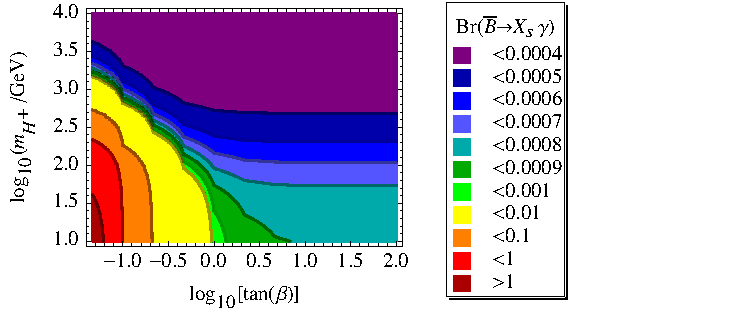
\includegraphics{THDMbsgplot.pdf}}
   \end{picture}
  }
  \caption{An illustration of the tabled values of ${\rm Br}(\bar{B}\to X_s\gamma)$ in dependence of the decadic logarithms of $\tan (\beta)$ and the charged Higgs mass.}
  \label{fig:THDMbsgplot}
\end{figure}

\textbf{$B^-\to \tau \bar{\nu}$ decays}\\

We take the formula from \cite{Hou:1992sy}: the SM branching ratio is proportional to the squared Wilson coefficient, to which we add the THDM contribution

\begin{align}
%CMbtaunu in the code
 C_? &= -4 \frac{G_F}{\sqrt{2}} V_{ub} m_{B^+}^2 \frac{\tan ^2 (\beta)}{m_{H^+}^2}. \nonumber
\end{align}




\begin{table}
  \centering
  \begin{tabular}{|l|l|c|c|c|c|c|}
    \hline
    \textbf{Theory observable} & \textbf{\HEPfit name} & \textbf{SM} & \textbf{THDM} & \textbf{MSSM} & \textbf{Dim-6} & \textbf{MHC} \\
    \hline
	$\lambda_1$ & \tt{lambda1} & & \checkmark & & &\\
    \hline
	$\lambda_2$ & \tt{lambda2} & & \checkmark & & &\\
    \hline
	$\lambda_3$ & \tt{lambda3} & & \checkmark & & &\\
    \hline
	$\lambda_4$ & \tt{lambda4} & & \checkmark & & &\\
    \hline
	$\lambda_5$ & \tt{lambda5} & & \checkmark & & &\\
    \hline
	\texttt{globalminimum}\:[GeV$^4$] & \tt{globalminimum} & & \checkmark & & &\\
    \hline
	\tt{positivity1} & \tt{positivity1} & & \checkmark & & &\\
    \hline
	\tt{positivity2} & \tt{positivity2} & & \checkmark & & &\\
    \hline
	$\Lambda^{\text{even}}_{21+}$ & \tt{unitarity1} & & \checkmark & & &\\
    \hline
	$\Lambda^{\text{even}}_{21-}$ & \tt{unitarity2} & & \checkmark & & &\\
    \hline
	$\Lambda^{\text{even}}_{01+}$ & \tt{unitarity3} & & \checkmark & & &\\
    \hline
	$\Lambda^{\text{even}}_{01-}$ & \tt{unitarity4} & & \checkmark & & &\\
    \hline
	$\Lambda^{\text{even}}_{00+}$ & \tt{unitarity5} & & \checkmark & & &\\
    \hline
	$\Lambda^{\text{even}}_{00-}$ & \tt{unitarity6} & & \checkmark & & &\\
    \hline
	$\Lambda^{\text{odd}}_{21}$ & \tt{unitarity7} & & \checkmark & & &\\
    \hline
	$\Lambda^{\text{odd}}_{20}$ & \tt{unitarity8} & & \checkmark & & &\\
    \hline
	$\Lambda^{\text{odd}}_{01+}$ & \tt{unitarity9} & & \checkmark & & &\\
    \hline
	$\Lambda^{\text{odd}}_{01-}$ & \tt{unitarity10} & & \checkmark & & &\\
    \hline
	$\Lambda^{\text{odd}}_{00+}$ & \tt{unitarity11} & & \checkmark & & &\\
    \hline
	$\Lambda^{\text{odd}}_{00-}$ & \tt{unitarity12} & & \checkmark & & &\\
    \hline
  \end{tabular}
  \caption{This table summarizes the theory observables of the models
    implemented in the code.}
  \label{tab:summarytheory}
\end{table}

\begin{table}
  \centering
  \begin{tabular}{|l|l|c|c|c|c|c|}
    \hline
    \textbf{Electroweak precision observable} & \textbf{\HEPfit name} & \textbf{SM} & \textbf{THDM} & \textbf{MSSM} & \textbf{Dim-6} & \textbf{MHC} \\
    \hline
	$\Delta S$ & \tt{DeltaS} & & \checkmark & & &\\
    \hline
	$\Delta T$ & \tt{DeltaT} & & \checkmark & & &\\
    \hline
	$\Delta U$ & \tt{DeltaU} & & \checkmark & & &\\
    \hline
  \end{tabular}
  \caption{This table summarizes the electroweak precision observables of the models
    implemented in the code.}
  \label{tab:summaryewpo}
\end{table}

\begin{table}
  \centering
  \begin{tabular}{|l|l|c|c|c|c|c|}
    \hline
    \textbf{Higgs observable} & \textbf{\HEPfit name} & \textbf{SM} & \textbf{THDM} & \textbf{MSSM} & \textbf{Dim-6} & \textbf{MHC} \\
    \hline
	$\Gamma_h$ [GeV] & \tt{a} & & \checkmark & & &\\
    \hline
	$r^{(h)}_{\gamma\gamma}$ & \tt{a} & & \checkmark & & &\\
    \hline
	$r^{(h)}_{Z\gamma}$ & \tt{a} & & \checkmark & & &\\
    \hline
	$r^{(h)}_{gg}$ & \tt{a} & & \checkmark & & &\\
    \hline
	$\mu_{\text{\tiny{ggF+tth}}}(h\to bb)$ & \tt{a} & & \checkmark & & &\\
    \hline
	$\mu_{\text{\tiny{VBF+Vh}}}(h\to bb)$ & \tt{a} & & \checkmark & & &\\
    \hline
	$\mu_{\text{\tiny{ggF+tth}}}(h\to WW)$ & \tt{a} & & \checkmark & & &\\
    \hline
	$\mu_{\text{\tiny{VBF+Vh}}}(h\to WW)$ & \tt{a} & & \checkmark & & &\\
    \hline
	$\mu_{\text{\tiny{ggF+tth}}}(h\to \tau \tau)$ & \tt{a} & & \checkmark & & &\\
    \hline
	$\mu_{\text{\tiny{VBF+Vh}}}(h\to \tau \tau)$ & \tt{a} & & \checkmark & & &\\
    \hline
	$\mu_{\text{\tiny{ggF+tth}}}(h\to ZZ)$ & \tt{a} & & \checkmark & & &\\
    \hline
	$\mu_{\text{\tiny{VBF+Vh}}}(h\to ZZ)$ & \tt{a} & & \checkmark & & &\\
    \hline
	$\mu_{\text{\tiny{ggF+tth}}}(h\to \gamma\gamma)$ & \tt{a} & & \checkmark & & &\\
    \hline
	$\mu_{\text{\tiny{VBF+Vh}}}(h\to \gamma\gamma)$ & \tt{a} & & \checkmark & & &\\
    \hline
	$\Gamma^{(H)}_{\text{tot}}$ [GeV] & \tt{a} & & \checkmark & & &\\
    \hline
	$\Gamma^{(H)}_{\gamma\gamma}$ [GeV] & \tt{a} & & \checkmark & & &\\
    \hline
	$\Gamma^{(H)}_{Z\gamma}$ [GeV] & \tt{a} & & \checkmark & & &\\
    \hline
	$\Gamma^{(H)}_{gg}$ [GeV] & \tt{a} & & \checkmark & & &\\
    \hline
	${\rm Br}(H\to hh)$ & \tt{a} & & \checkmark & & &\\
    \hline
	${\rm Br}(H\to AA)$ & \tt{a} & & \checkmark & & &\\
    \hline
	${\rm Br}(H\to H^+H^-)$ & \tt{a} & & \checkmark & & &\\
    \hline
	${\rm Br}(H\to AZ)$ & \tt{a} & & \checkmark & & &\\
    \hline
	${\rm Br}(H\to H^\pm W^\mp)$ & \tt{a} & & \checkmark & & &\\
    \hline
	${\rm Br}(H\to t\bar{t})$ & \tt{a} & & \checkmark & & &\\
    \hline
%%%
%%%\begin{align}
%%%& \sigma ^{(H)}_{\text{\tiny{ggF}}} \cdot {\rm Br}(H\to \tau \tau ) , \quad \sigma ^{(H)}_{\text{\tiny{bbH}}} \cdot {\rm Br}(H\to \tau \tau ), \quad\sigma ^{(H)}_{\text{\tiny{pp}}} \cdot {\rm Br}(H\to \gamma \gamma ) , \quad \sigma ^{(H)}_{\text{\tiny{ggF}}} \cdot {\rm Br}(H\to \gamma \gamma ), \nonumber \\ %C8
%%%%& \sigma ^{(H)}_{\text{\tiny{ggF}}} \cdot {\rm Br}(H\to tt) \nonumber \\ %A8
%%%& \sigma ^{(H)}_{\text{\tiny{bbH}}} \cdot {\rm Br}(H\to bb), \quad \sigma ^{(H)}_{\text{\tiny{ggF}}} \cdot {\rm Br}(H\to WW) , \quad , \quad \sigma ^{(H)}_{\text{\tiny{ggF}}} \cdot {\rm Br}(H\to ZZ), \nonumber \\ %A8
%%%& \sigma ^{(H)}_{\text{\tiny{VBF}}} \cdot {\rm Br}(H\to ZZ), \quad \sigma ^{(H)}_{\text{\tiny{pp}}} \cdot {\rm Br}(H\to VV) /  (\sigma ^{(H)}_{\text{\tiny{pp}}} \cdot {\rm Br}(H\to VV) )_{SM}, \nonumber \\ %C8
%%%& \sigma ^{(H)}_{\text{\tiny{ggF}}} \cdot {\rm Br}(H\to hh) , \quad \sigma ^{(H)}_{\text{\tiny{ggF}}} \cdot {\rm Br}(H\to hh \to (bb)(\tau \tau )), \nonumber \\ %C8
%%%& \sigma ^{(H)}_{\text{\tiny{pp}}} \cdot {\rm Br}(H\to hh \to (bb)(bb)) , \quad \sigma ^{(H)}_{\text{\tiny{pp}}} \cdot {\rm Br}(H\to hh \to (\gamma \gamma )(bb)) \nonumber %C8
%	$\sigma_{\text{ggH}}\!\cdot\! BR(H\!\to\! \tau\tau)$ [pb] & \tt{a} & & \checkmark & & &\\
%    \hline
%	$\sigma_{\text{bbH}}\!\cdot\! BR(H\!\to\! \tau\tau)$ [pb] & \tt{a} & & \checkmark & & &\\
%    \hline
%	$\sigma_{\text{ggH}}\!\cdot\! BR(H\!\to\! \gamma\gamma)$ [pb] & \tt{a} & & \checkmark & & &\\
%    \hline
%	$\mu_{\text{ggH}}(H\!\to\! ZZ)$ [pb] & \tt{a} & & \checkmark & & &\\
%    \hline
%	$\sigma_{\text{ggH}}\!\cdot\! BR(H\!\to\! WW)$ [pb] & \tt{a} & & \checkmark & & &\\
%    \hline
	$R^{(H)}_\text{\tiny Gauss} \left( \sigma ^{(H)}_{\text{\tiny{VBF}}} \cdot {\rm Br}(H\to WW)\right) $ & \tt{Robs\_VBF\_H\_WW\_ATLAS} & & \checkmark & & &\\
    \hline
%	$\sigma_{\text{ggH}}\!\cdot\! BR(H\!\to\! hh)$ [pb] & \tt{a} & & \checkmark & & &\\
%    \hline
%	$\sigma_{\text{ggH}}\!\cdot\! BR(H\!\to\! hh\!\to\! b\bar{b}\tau\tau)$ [pb] & \tt{a} & & \checkmark & & &\\
%    \hline
%	$\sigma_{\text{ppH}}\!\cdot\! BR(H\!\to\! hh\!\to\! b\bar{b}b\bar{b})$ [pb] & \tt{a} & & \checkmark & & &\\
%    \hline
%	$\sigma_{\text{ppH}}\!\cdot\! BR(H\!\to\! hh\!\to\! \gamma\gamma b\bar{b})$ [pb] & \tt{a} & & \checkmark & & &\\
%    \hline
%	$\sigma_{\text{ppH}}\!\cdot\! BR(H\!\to\! t\bar{t})$ [pb] & \tt{a} & & \checkmark & & &\\
%    \hline
%	$\sigma_{\text{bbH}}\!\cdot\! BR(H\!\to\! b\bar{b})$ [pb] & \tt{a} & & \checkmark & & &\\
%    \hline
%	$\Gamma_A$\:[GeV] & $36.29233235$ & $36.91...$ & $36.29233685502$ & $-1.24\cdot 10^{-7}$\\
%	$\Gamma^{(A)}_{\gamma\gamma}$\:[keV] & $115.7310131$ & ? & $115.730932428$ & $6.97\cdot 10^{-7}$\\
%	$\Gamma^{(A)}_{Z\gamma}$\:[keV] & $26.45319592$ & -- & $26.4531773199$ & $7.03\cdot 10^{-7}$\\
%	$\Gamma^{(A)}_{gg}$\:[MeV] & $34.54622361$ & ? & $34.5470976006$ & $-2.53\cdot 10^{-5}$\\
%	${\rm Br}(A\!\to\! HZ)$\:[\%] & $0$ & $0$ & $0$ & $0$\\
%	${\rm Br}(A\!\to\! hZ)$\:[\%] & $0.2266869081$ & $0.2226...$ & $0.226687$ & $1.24\cdot 10^{-7}$\\
%	${\rm Br}(A\!\to\! H^\pm W^\mp)$\:[\%] & $55.35440718$ & $54.58...$ & $55.35440031326$ & $1.24\cdot 10^{-7}$\\
%	${\rm Br}(A\!\to\! t\bar{t})$\:[\%] & $44.245441475$ & ? & $44.24543599800$ & $1.24\cdot 10^{-7}$\\
%	$\sigma_{\text{ggA}}\!\cdot\! BR(A\!\to\! \tau\tau)$\:[ab] & $11.963695367$ & $11.74...$ & $11.40262184364$ & $4.69\cdot 10^{-2}$\\
%	$\sigma_{\text{bbA}}\!\cdot\! BR(A\!\to\! \tau\tau)$\:[zb] & $20.73324124$ & $20.36...$ & $18.01168794027$ & $1.31\cdot 10^{-1}$\\
%	$\sigma_{\text{ggA}}\!\cdot\! BR(A\!\to\! \gamma\gamma)$\:[ab] & $0.4310178090807$ & $1.262...$ & $0.410782470058$ & $4.69\cdot 10^{-2}$\\
%	$\sigma_{\text{ggA}}\!\cdot\! BR(A\!\to\! hZ\!\to\! b\bar{b}\ell\ell)$\:[ab] & $12.3003$ & $12.43...$ & $12.965$ & $-5.40\cdot 10^{-2}$\\
%	$\sigma_{\text{ggA}}\!\cdot\! BR(A\!\to\! hZ\!\to\! b\bar{b}Z)$\:[fb] & $0.182795$ & $0.1847...$ & $0.192599$ & $-5.36\cdot 10^{-2}$\\
%	$\sigma_{\text{ggA}}\!\cdot\! BR(A\!\to\! hZ\!\to\! \tau\tau \ell\ell)$\:[ab] & $2.02201$ & $1.787...$ & $2.13012$ & $-5.35\cdot 10^{-2}$\\
%	$\sigma_{\text{ggA}}\!\cdot\! BR(A\!\to\! hZ\!\to\! \tau\tau Z)$\:[ab] & $20.0219$ & $17.70...$ & $21.0958$ & $-5.36\cdot 10^{-2}$\\
%	$\sigma_{\text{ppA}}\!\cdot\! BR(A\!\to\! t\bar{t})$\:[fb] & $59.9075$ & $60.87...$ & $57.08623$ & $4.71\cdot 10^{-2}$\\
%	$\sigma_{\text{bbA}}\!\cdot\! BR(A\!\to\! b\bar{b})$\:[ab] & $0.16017$ & $0.1573...$ & $0.13916214$ & $1.31\cdot 10^{-1}$\\
  \end{tabular}
  \caption{This table summarizes the Higgs observables of the models
    implemented in the code.}
  \label{tab:summaryhiggs}
\end{table}

\begin{table}
  \centering
  \begin{tabular}{|l|l|c|c|c|c|c|}
    \hline
    \textbf{Flavour observable} & \textbf{\HEPfit name} & \textbf{SM} & \textbf{THDM} & \textbf{MSSM} & \textbf{Dim-6} & \textbf{MHC} \\
    \hline
	${\rm Br}(\bar{B}\to X_s\gamma)$ & \tt{BR\_bsgamma} & \checkmark & & & &\\
    \hline
	${\rm Br}(\bar{B}\to X_s\gamma)$ & \tt{B\_BtoXsgammaTHDM} & & \checkmark & & &\\
    \hline
	$\Delta m_{B_s}$ & \tt{DmBs} & \checkmark & \checkmark & & &\\
    \hline
	${\rm Br}(B^-\to \tau \bar{\nu})$ & \tt{btaunu} & \checkmark & \checkmark & & &\\
    \hline
  \end{tabular}
  \caption{This table summarizes the flavour observables of the models
    implemented in the code.}
  \label{tab:summaryflavour}
\end{table}

%%%%%%%%%%%%%%%%%%%%%%%%%%%%%%%%%%%%%
\section{Code Description}
\label{sec:Code}
%%%%%%%%%%%%%%%%%%%%%%%%%%%%%%%%%%%%%

L+M+E, Ayan



%%%%%%%%%%%%%%%%%%%%%%%%%%%%%%%%%%%%%
\section{Usage and Examples}
\label{sec:Usage}
%%%%%%%%%%%%%%%%%%%%%%%%%%%%%%%%%%%%%

Ayan



%%%%%%%%%%%%%%%%%%%%%%%%%%%%%%%%%%%%%
\section{Comparison with Other Codes}
\label{sec:Comparison}
%%%%%%%%%%%%%%%%%%%%%%%%%%%%%%%%%%%%%

%%%%%%%%%%%%%%%%%%%%%%%%
\subsection{Comparison with ZFITTER}
\label{sec:ZFitter}
%%%%%%%%%%%%%%%%%%%%%%%%

Satoshi

%%%%%%%%%%%%%%%%%%%%%%%%
\subsection{Comparison with UTfit}
\label{sec:UTfit}
%%%%%%%%%%%%%%%%%%%%%%%%

L+M+E

%%%%%%%%%%%%%%%%%%%%%%%%
\subsection{Comparison with JDBM}
\label{sec:JDBM}
%%%%%%%%%%%%%%%%%%%%%%%%

Jorge

%%%%%%%%%%%%%%%%%%%%%%%%
\subsection{Comparison with SuSEFlav}
\label{sec:Debtosh}
%%%%%%%%%%%%%%%%%%%%%%%%

Debtosh

%%%%%%%%%%%%%%%%%%%%%%%%
\subsection{More comparisons....}
\label{sec:more}
%%%%%%%%%%%%%%%%%%%%%%%%

Otto


\cite{hep-ph/9412201,hep-ph/9908433,hep-ph/0507146,1302.1395}.


\acknowledgments
M.C. is associated to the Dipartimento di Fisica, Universit\`a di Roma
Tre. E.F. and L.S. are associated to the Dipartimento di Fisica,
Universit\`a di Roma ``La Sapienza''. We acknowledge partial support
from ERC Ideas Starting Grant n.~279972 ``NPFlavour'' and ERC Ideas
Advanced Grant n.~267985 ``DaMeSyFla''.

\bibliography{HEPfit-1.0}

\end{document}
